\chapter{Context}
\section{Background on PAKEs}
\subsection{What is a PAKE?}
\glspl{pake} are interactive, two party cryptographic protocols where each party shares knowledge of a password (a low entropy secret) and seeks to obtain a strong shared key e.g. for use later with a symmetric cipher. Critically an eavesdropper who can listen in two all messages of the key negotiation cannot learn enough information to bruteforce the password. Another way of phrasing this is that brute force attacks on the key must be "\glslink{ocrypto}{online}".

\medskip
There are two main types of \gls{pake} algorithm - \glspl{apake} and \glspl{bpake}.
\begin{itemize}
  \item \glspl{bpake} are \glspl{pake} where both parties share knowledge of the same secret password.
  \item \glspl{apake} are \glspl{pake} where one party has the password and the other has a "\gls{veri}" which is computed via a one-way function from the secret password.
\end{itemize}

\begin{figure}[H]
  \centering
  \begin{tikzpicture}
    \node[alice,minimum size=1.5cm] at (0,0) {Alice};
    \node[scale=0.03] at (1,0.5) {
\includegraphics{key.png}};
    \node[bob,mirrored,minimum size=1.5cm] at (5,0) {Bob};
    \node[scale=0.03] at (4,0.5) {
\includegraphics{key.png}};
    \node[alice,minimum size=1.5cm] at (7,0) {Alice};
    \node[scale=0.03] at (8,0.5) {
\includegraphics{key.png}};
    \node[bob,mirrored,minimum size=1.5cm] at (12,0) {Bob};
    \node[scale=0.03] at (11,0.5) {
\includegraphics{shuffled_key.png}};
    \draw (6,1.3) -- (6,-2.3);
    \draw (2.5,-2) node {Balanced PAKE};
    \draw (9.5,-2) node {Augmented PAKE};
  \end{tikzpicture}

  \caption{An illustration of the difference between \glspl{apake} and \glspl{bpake}}
  \label{fig:pake_compare}
\end{figure}

\clearpage

\subsection{A brief history of PAKE algorithms}
The first \gls{pake} algorithm was Bellovin and Merritt's \gls{eke} scheme\cite{eke}.
It works using a mix of \gls{symcrypto} and \gls{asymcrypto} to perform a key exchange.
This comes with many challenges and subtle mistakes that are easy to make;
primarily for the security of the system whatever is encrypted by the shared secret key(P) must be indistinguishable from random data.
Otherwise an attacker can determine whether their guess at a trial decryption is valid.
The \gls{rsa} variant of \gls{eke} has this issue - the \gls{rsa} parameter $e$ is what is encrypted and sent in the first message.
For \gls{rsa} all valid values of $e$ are odd, so this would prevent it being used.
This is solved by adding $1$ to $e$ with a $50\%$ chance.
\Cref{fig:eke-rsa} shows this protocol in full. While many of the initial variants on \gls{eke} have been shown to flawed/vulnerable, later variants have made it into real world use, such as in \gls{eap}\cite{eap} where it is available as \gls{eap}-\gls{eke}\cite{eap-eke}.
In \cref{chap:appendix-eke} you can find a Python implementation of this scheme

\subsubsection{An Aside on Notation}
\begin{itemize}
  \item $\shortleftarrow$: Assignment - $x \shortleftarrow \ 5$ means x is assigned a value of 5.
  \item $\cryptoSample$: Sampling from a given set - $x \cryptoSample \ \mathbb{R}$ means to choose $x$ at random from the set of real numbers.
\end{itemize}

\begin{figure}[H]
  \centering

  \begin{tabular}{ |c|c|l| }
    \hline
    Shared Parameter & Secret & Explanation \\
    \hline
    $P$ & yes & the shared password \\ \hline
  \end{tabular}

  \caption{\gls{eke} shared parameters}
  \label{fig:eke-shared-params}
\end{figure}

\begin{figure}[H]
  \pseudocodeblock[head=EKE-RSA]{
    \textbf{Alice} \< \< \textbf{Bob} \\[0.1\baselineskip][\hline]
    \< \< \\[-0.5\baselineskip]
    Ea \gets (e, n) \< \< \\
    b \sample \bin \< \sendmessageright*{A,P(e + b),n} \< Ea \gets (e, n)\\ 
    challenge_A \sample \ZZ_n \< \sendmessageleft*{P(Ea(R))} \< R \sample \text{Keyspace}\\ 
    \< \sendmessageright*{R(challenge_A)} \< challenge_B \sample \ZZ_n \\
    \text{verify } challenge_A \< \sendmessageleft*{R(challenge_A, challenge_B)} \< \\
    \< \sendmessageright*{R(challenge_B)} \< \text{verify } challenge_B
  }

  \caption{Implementing \gls{eke} using \gls{rsa}}
  \label{fig:eke-rsa}
\end{figure}

\clearpage

\subsubsection{SPAKE}
\glslink{spake}{SPAKE1} and \glslink{spake}{SPAKE2} are \glspl{bpake}' which were introduced slightly later on by Michel Abdalla and David Pointcheval\cite{spake} as variations on \gls{eke}.
\glslink{spake}{SPAKE2} and \glslink{spake}{SPAKE2} are very similar so we will just explore \glslink{spake}{SPAKE2} as we are more interested in \glslink{ocrypto}{online} algorithms.
\glslink{spake}{SPAKE2} is also 
\gls{spake} differs from EKE in the following ways:

\begin{enumerate}
  \item The encryption function is replaced by a simple one-time pad.
  \item The \gls{asymcrypto} is provided by \gls{dh}
  \item There is no explicit mutual authentication phase where challenges are exchanged.
    This has the advantage of reducing the number of messages that need to be sent.
\end{enumerate}

\begin{figure}[H]
  \centering

  \begin{tabular}{ |c|c|p{0.6\linewidth}| }
    \hline
    Shared Parameter & Secret & Explanation \\
    \hline
    $pw$ & yes & the shared password encoded as an element of $\ZZ_p$ \\ \hline
    $\GG$ & no & the mathematical group in which we will perform all opertions \\  \hline
    $g$ & no & the generator of $\GG$ \\ \hline
    $p$ & no & the \gls{safeprime} which defines the finite field for all operations in $\GG$ \\ \hline
    $M$ & no & an element in $\GG$ associated with user $A$ \\ \hline
    $N$ & no & an element in $\GG$ associated with user $B$ \\ \hline
    $H$ & no & a secure hash function \\ \hline
  \end{tabular}

  \caption{\gls{spake} shared parameters}
  \label{fig:spake-shared-params}
\end{figure}

\begin{figure}[H]
  \pseudocodeblock[head=SPAKE2]{
    \textbf{Alice} \< \< \textbf{Bob} \\[0.1\baselineskip][\hline]
    \< \< \\[-0.5\baselineskip]
    x \sample \ZZ_p \< \< y \sample \ZZ_p \\
    X \gets g^x \< \< Y \gets g^y \\
    X^* \gets X \cdot M^{pw} \< \< Y^* \gets X \cdot N^{pw} \\
    \< \sendmessageright*{X^*} \< \\
    \< \sendmessageleft*{Y^*} \< \\
    K_A \gets (Y^* / N^{pw})^x \< \< K_B \gets (X^* / M^{pw})^y \\
    SK_A \gets H(A, B, X^*, Y^*, Ka) \< \< SK_B \gets H(A, B, X^*, Y^*, Kb)
  }

  \caption{SPAKE2 Protocol}
  \label{fig:spake2}
\end{figure}

\clearpage

\subsubsection{SRP}
Finally we will look at \gls{srp} an \gls{apake} first published in 1998, unlike \glslink{spake}{SPAKE2} it is not a modification of \gls{eke}.
\gls{srp} has gone through many revisions, at time of writing \glslink{srp}{SRP6a} is the latest version.
\gls{srp} is likely the most used \gls{pake} protocol in the world due to it's use in Apple's iCloud Keychain\cite{apple-keychain-srp} and it's availability as a \gls{tls} ciphersuite\cite{tls-srp}.
However it is quite weird for what it does and there is no security proof for it\cite{srp-blog}. An implementation of the protocol in Python can be found in \cref{chap:appendix-srp}.

\begin{figure}[H]
  \centering

  \begin{tabular}{ |c|c|p{0.7\linewidth}| }
    \hline
    Parameter & Secret & Explanation \\
    \hline
    $v$ & yes & the \gls{veri}\label{text:srp-verifier-generation} stored by the server: $v=g^{H(s,I,P)}$ \\ \hline
    $P$ & yes & the user's password \\ \hline
    $I$ & no & the user's name \\ \hline
    $g$ & no & the generator of $\GG$ \\ \hline
    $p$ & no & the \gls{safeprime} which defines the finite field for all operations in $\GG$ \\ \hline
    $H$ & no & a secure hash function \\ \hline
  \end{tabular}

  \caption{\gls{srp} parameters}
  \label{fig:srp-shared-params}
\end{figure}

\begin{figure}[H]
  \pseudocodeblock[head=SRP]{
    \textbf{Alice} \< \< \textbf{Bob} \\[0.1\baselineskip][\hline]
    \< \< \\[-0.5\baselineskip]
    a \sample \{1 \dots n - 1\} \< \sendmessageright*{I} \< s,v \gets \text{lookup}(I)\\
    x \gets H(s, I, P) \< \sendmessageleft*{s} \< b \sample \{1 \dots n - 1\}\\
    A \gets g^a \< \sendmessageright*{A} \< B \gets 3v + g^b \\
    u \gets H(A, B) \< \sendmessageleft*{B} \< u \gets H(A, B)\\
    S \gets (B - 3g^x)^{a+ux}\< \< S \gets (Av^u)^b\\
    M_1 \gets H(A,B,S) \< \sendmessageright*{M_1} \< \text{verify } M_1\\
    \text{verify } M_2 \< \sendmessageleft*{M_2} \< M_2 \gets H(A,M_1,S)\\
    K \gets H(s)\< \< K \gets H(S)
  }

  \caption{SRP-6 Protocol}
  \label{fig:srp}
\end{figure}

\clearpage

\section{Elliptic Curve Cryptography}
Many modern Cryptograhpic protocols make use of a mathematical object known as an elliptic curve.
First proposed in 1985 independently by Neal Koblitz\cite{ecc-first-use-koblitz} and Victor S. Miller\cite{ecc-first-use-miller}.
Elliptic curves are attractive to cryptographers as they maintain a very high level of strength at smaller key sizes, this allows for protocols to consume less bandwidth, less memory and execute faster\cite{state-of-ecc}.
To illustrate just how great the size savings are - \gls{nist} suggests that an elliptic curve key of just 256 bits provides the same level of security as an \gls{rsa} key of 3072 bits\cite{nist-ecc-reqs}.

\subsection{But what actually is an elliptic curve?}
With regards to Cryptography elliptic curves tend to come in one of two forms:
\begin{itemize}
  \item Short Weierstra\ss{} Form: $y^2 = x^3 + ax + b$
  \item Montgomery Form: $by^2 = x^3 + ax^2 + x$
\end{itemize}

\begin{figure}
  \centering
  \begin{tikzpicture}[thick,>=latex]
    \begin{scope}
      \draw[<->,gray] (-3,0) -- (3,0) node[right] {$x \in \mathbb{R}$};
      \draw[<->,gray] (0,-3) -- (0,3) node[above] {$y \in \mathbb{R}$};
      \draw[thick, name path=curve, every plot/.style={smooth}] plot[id=weierstrass-curve-1, raw gnuplot] function {
        f(x,y) = y**2 - (x**3 - 2.5*x + 1);
        set xrange [-3:3];
        set yrange [-3:3];
        set view 0,0;
        set isosample 50,50;
        set cont base;
        set cntrparam levels incre 0,0.1,0;
        unset surface;
        splot f(x,y);
      };
    \end{scope}

    \node at (0,-4) {$y^2 = x^3 - 2 x - 1$ over $\mathbb{R}$};
    \node at (0,-5) {Short Weierstra\ss{} Form};

    \begin{scope}[shift={(8,0)}]
      \draw[<->,gray] (-3,0) -- (3,0) node[right] {$x \in \mathbb{R}$};
      \draw[<->,gray] (0,-3) -- (0,3) node[above] {$y \in \mathbb{R}$};
      \draw[thick, name path=curve, every plot/.style={smooth}] plot[id=montgomery-curve-1, raw gnuplot] function {
        f(x,y) = 2*y**2 - (x**3 - 3*x - x);
        set xrange [-3:3];
        set yrange [-3:3];
        set view 0,0;
        set isosample 50,50;
        set cont base;
        set cntrparam levels incre 0,0.1,0;
        unset surface;
        splot f(x,y);
      };
    \end{scope}

    \node at (8,-4) {$2 y^2 = x^3 - 3 x^2 - x$ over $\mathbb{R}$};
    \node at (8,-5) {Montgomery Form};
  \end{tikzpicture}

  \caption{Elliptic curves over $\ZZ_{89}$, Inspired by TikZ for Cryptographers\cite{tikz-crypto}}
\end{figure}

Weierstra\ss{} form is special as it is the general case for all elliptic curves, meaning all elliptic curves can be expressed as a Weierstra\ss{} curve.
This property means that it is commonly used for expressing various curves.
Montgomery form isn't quite as flexible, however it is favourable because it leads to significantly faster multiplication and addition operations via Montgomery's ladder\cite{montgom-ladder}.

\subsection{How do we do Cryptography with curves?}
To perform Cryptography with elliptic curves we need to define an "\gls{abgroup}" to work in.
An \gls{abgroup} is a group whose group operation is also commutative, for example the addition operator over the integers: ($+$, $\ZZ$) is an \gls{abgroup}.
\glspl{abgroup} form the basis of many modern Cryptographic algorithms, a \gls{dh} key exchange can be performed in any \gls{abgroup} for instance.

To define an abelian group over our elliptic curves we need a set $G$, our set will be the set of integer points on the curve mod a prime $p$ - $\{ x | x \in \ZZ_p \text{ and } \exists (y \in \ZZ_p) [By^2 = x^3 + Ax^2 + x] \}$.
It is helpful to visualalise this so lets take our curves from before and see how they look in a small group - $\ZZ_{89}$.

\begin{center}
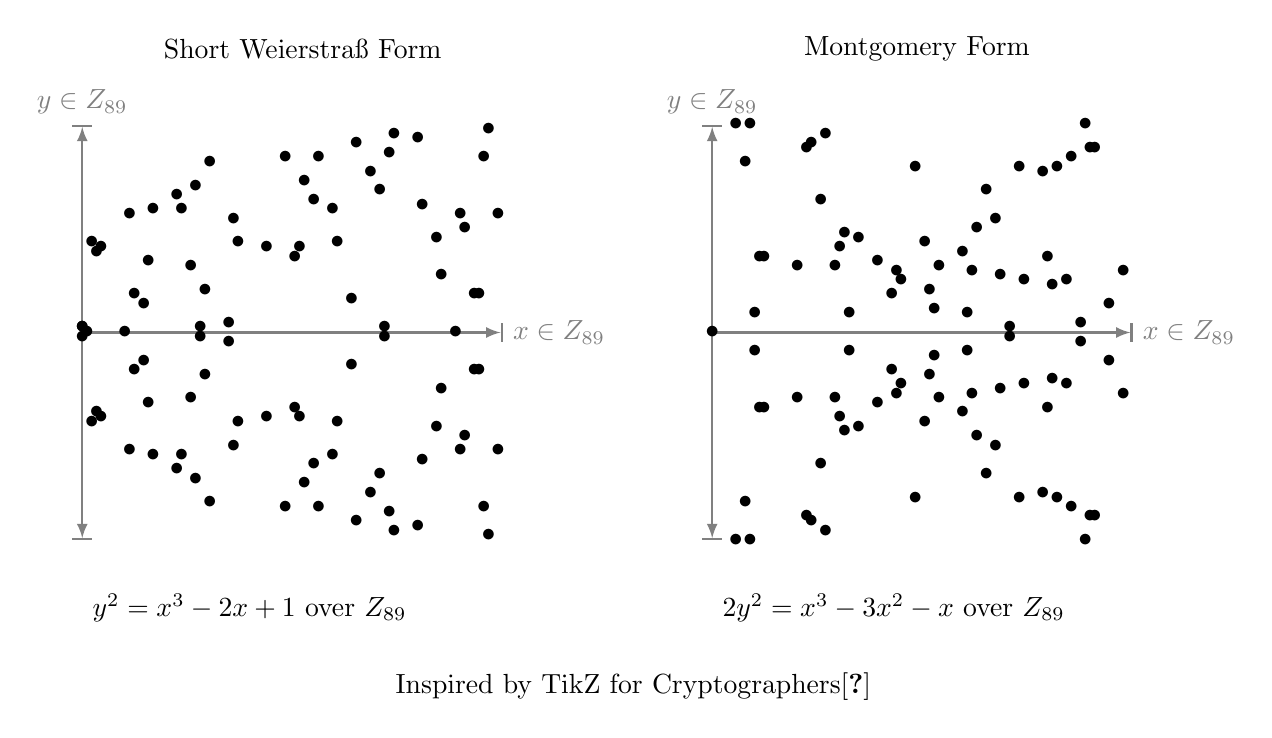
\begin{tikzpicture}[thick,>=latex]
  % Generate list of points with Sage:
  % sage: E = EllipticCurve(Integers(89), [-2,1])
  % sage: points = [(int(P[0]), int(P[1])) for P in E.points()]
  % yes this is suspect as fuck but it all works because modular arithmetic 🙃
  % sage: print([(x,y if y <= 44 else y-89) for x,y in points])
  \begin{scope}[scale=.060]
    \draw[|<->|,gray] (0,-44) -- (0,44) node[above] {$y \in \mathbb{Z}_{89}$};
    \draw[->|,gray] (0,0) -- (89,0) node[right] {$x \in \mathbb{Z}_{89}$};
    \foreach \point in {
      (0, 1), (0, 1), (0, -1), (1, 0), (2, 19), (2, -19), (3, 17), (3, -17), (4, 18), (4, -18), (9, 0), (10, 25),
      (10, -25), (11, 8), (11, -8), (13, 6), (13, -6), (14, 15), (14, -15), (15, 26), (15, -26), (20, 29), (20, -29),
      (21, 26), (21, -26), (23, 14), (23, -14), (24, 31), (24, -31), (25, 1), (25, -1), (26, 9), (26, -9), (27, 36),
      (27, -36), (31, 2), (31, -2), (32, 24), (32, -24), (33, 19), (33, -19), (39, 18), (39, -18), (43, 37),
      (43, -37), (45, 16), (45, -16), (46, 18), (46, -18), (47, 32), (47, -32), (49, 28), (49, -28), (50, 37),
      (50, -37), (53, 26), (53, -26), (54, 19), (54, -19), (57, 7), (57, -7), (58, 40), (58, -40), (61, 34),
      (61, -34), (63, 30), (63, -30), (64, 1), (64, -1), (65, 38), (65, -38), (66, 42), (66, -42), (71, 41),
      (71, -41), (72, 27), (72, -27), (75, 20), (75, -20), (76, 12), (76, -12), (79, 0), (80, 25), (80, -25),
      (81, 22), (81, -22), (83, 8), (83, -8), (84, 8), (84, -8), (85, 37), (85, -37), (86, 43), (86, -43),
      (88, 25), (88, -25)
    } {\node at \point {$\bullet$};}
  \end{scope}

  \node[right] at (0,-3.5) {$y^2 = x^3 - 2 x + 1$ over $\mathbb{Z}_{89}$};
  \node at (2.8,3.6) {Short Weierstra\ss{} Form};

  % Generate list of points with Python:
  % >>> f=lambda x,y: (int(2 * y**2) % 89) == ((x**3 -3*(x**2) - x) % 89)
  % >>> # yes this is suspect as fuck but it all works because modular arithmetic 🙃
  % >>> points = [(x,y if y <= 44 else y - 89) for x in range(89) for y in range(89) if f(x, y)]
  % >>> print(points)
  \begin{scope}[xshift=8cm,scale=.060]
    \draw[|<->|,gray] (0,-44) -- (0,44) node[above] {$y \in \mathbb{Z}_{89}$};
    \draw[->|,gray] (0,0) -- (89,0) node[right] {$x \in \mathbb{Z}_{89}$};
    \foreach \point in {
      (0, 0), (5, 44), (5, -44), (7, 36), (7, -36), (8, 44), (8, -44), (9, 4), (9, -4), (10, 16), (10, -16), (11, 16), (11, -16), (18, 14), (18, -14), (20, 39), (20, -39), (21, 40), (21, -40), (23, 28), (23, -28), (24, 42), (24, -42), (26, 14), (26, -14), (27, 18), (27, -18), (28, 21), (28, -21), (29, 4), (29, -4), (31, 20), (31, -20), (35, 15), (35, -15), (38, 8), (38, -8), (39, 13), (39, -13), (40, 11), (40, -11), (43, 35), (43, -35), (45, 19), (45, -19), (46, 9), (46, -9), (47, 5), (47, -5), (48, 14), (48, -14), (53, 17), (53, -17), (54, 4), (54, -4), (55, 13), (55, -13), (56, 22), (56, -22), (58, 30), (58, -30), (60, 24), (60, -24), (61, 12), (61, -12), (63, 1), (63, -1), (65, 35), (65, -35), (66, 11), (66, -11), (70, 34), (70, -34), (71, 16), (71, -16), (72, 10), (72, -10), (73, 35), (73, -35), (75, 11), (75, -11), (76, 37), (76, -37), (78, 2), (78, -2), (79, 44), (79, -44), (80, 39), (80, -39), (81, 39), (81, -39), (84, 6), (84, -6), (87, 13), (87, -13)
    } {\node at \point {$\bullet$};}
  \end{scope}

  \node at (10.6,3.6) {Montgomery Form};
  \node[right] at (8,-3.5) {$2y^2 = x^3 - 3x^2 - x$ over $\mathbb{Z}_{89}$};

  \node at (7,-4.5) {Inspired by TikZ for Cryptographers\cite{tikz-crypto}};
\end{tikzpicture}
\end{center}

This now looks very different to when we were looking at them in $\RR$, however it shows very clearly what the elements of our set look like. They are points in the 2d coordinate plane with a symmetry around the Y-axis, this is worth noting as it is the basis for forming our group's binary operator.

Lets build our binary operator, for this to work we need to define the notion of adding two points together, and it needs to be associative, have an inverse, have some notion of an "identity" and it needs to be commutative.
To start with we will define point addition using the "Chord rule" and then handle the edge cases.
The Chord rule

\begin{figure}[H]
  \centering
  \begin{tikzpicture}[scale=.555]

    \begin{scope}[xshift=0cm]
      \plotcurve{-2}{2}
      \draw[->, >=latex, thick] (-2.5,-1) -- ++(0,3.5) node[right] {$\mathcal{O}$};
      \node[below] at (0,-4) {Neutral element $\mathcal{O}$};
    \end{scope}

    \begin{scope}[xshift=7.5cm]
      \plotcurve{-2}{2}
      \draw[dashed, semithick, name path=vertical] (-1.25,2.5) -- ++(0,-5);
      \draw[name intersections={of=curve and vertical}] (intersection-1) node {$\bullet$} node[above left] {$P$}
      (intersection-2) node {$\bullet$} node[below left] {$-P$};
      \node[below] at (0,-4) {Inverse element $-P$};
    \end{scope}

    \begin{scope}[xshift=15cm]
      \plotcurve{-2}{2}
      \draw[thick, name path=chord] (-2.5,.5) -- (2.5,2.0);
      \draw[name intersections={of=curve and chord}] (intersection-1) node {$\bullet$} node[above left] {$P$}
      (intersection-2) node {$\bullet$} node[above right=-1pt] {$Q$}
      (intersection-3) node {$\bullet$} coordinate[name=mPQ];
      \draw[dashed, semithick, name path=vertical] (mPQ) ++(0,1) -- +(0,-5.5);
      \draw[name intersections={of=curve and vertical}] (intersection-2) node {$\bullet$} node[below left] {$P+Q$};
      \node[below, align=center] at (0,-4) {Addition $P+Q$ \\ ``Chord rule''};
    \end{scope}

    \begin{scope}[xshift=22.5cm]
      \plotcurve[thick, tangent=0.265, every plot/.style={sharp plot}]{-2}{2}
      \draw[thick, use tangent, name path=chord] (-.6,0) -- (1.5,0);
      \draw[name intersections={of=curve and chord}] (intersection-1) node {$\bullet$} node[above] {$P$}
      (intersection-2) node {$\bullet$} coordinate[name=mPQ];
      \draw[dashed, semithick, name path=vertical] (mPQ) ++(0,1) -- +(0,-5.0);
      \draw[name intersections={of=curve and vertical}] (intersection-2) node {$\bullet$} node[below left] {$2P$};
      \node[below, align=center] at (0,-4) {Doubling $P+P$ \\ ``Tangent rule''};
    \end{scope}

  \end{tikzpicture}
  \caption{Elliptic Curve Group Operations, reproduced from TikZ for Cryptographers\cite{tikz-crypto}}
  \label{fig:point-add-rules}
\end{figure}

\section{Modern PAKEs}
\section{AuCPace}
\section{Who are RustCrypto?}
